\documentclass[11pt]{article}
\usepackage{graphicx}
\usepackage{listings}
\usepackage[margin=1in]{geometry}
\usepackage{placeins}
\usepackage{float}
\lstset{language=python}
\usepackage{indentfirst}

\author{Group 9: Kofi Otseidu, Manav Trivedi, Andrew Smith}
\title{How Does Cost Affect Officer Behavior?}

\begin{document}
\maketitle


\section{Introduction}
Our goal in this project was to attempt to quantify the effect of cost, including an officer's salary as well as settlements they were involved in, on officer behavior. Do settlements deter cops from getting into trouble? Does having a high or low salary make an officer more likely to get into trouble? Does the neighborhood wealth have an effect on officer behavior? These are some of the questions we wanted to get at with access to the Chicago Police Department's complaints database, as well as a database of settlements the police were involved in.

Ultimately we cannot know what is in each individual officer's heart, but looking at the data can give us some idea of how to both prevent bad behavior in the first place, and also reward good officers most effectively. It also gives us insight into community interactions, particularly as Chicago has a diverse range of neighborhood wealth.


\section{Description and Summarization}
The first checkpoint that we worked on was Description and Summarization. Here we worked mainly on PostgreSQL. There were three questions that we wanted to answer through this checkpoint and we’ll go over them one at a time.

The first question that we wanted to get some clarity about was whether there is any significant differences in the average salary of the officers in each district in Chicago. We postulated that if there were a difference in the salaries of the officers ranging from district to district, it could be a factor leading to their behavior and affect the number of allegations against them. What we found was that the average salaries of the officers around the city was almost the same. In 2017, the police officers in Chicago received a salary of around \$90k and there was no significant difference in this number between the districts. It is interesting to look at some of the specialized units like the mounted or canine units and compare to the base police officer salary. Initially we had wondered whether officers would be paid more in nicer districts, possibly to cover the cost of living there, or whether they might be paid more in more dangerous districts. Neither seems to be the case, which makes sense assuming they all fall under one governing body, which they do. It would probably not be ideal to incentivize moving districts too often.

The second question was to summarize the amount of allegations per district in Chicago and find out which areas had the highest number of allegations or interactions with the police. The result showed that a few districts, namely the Loop and Austin, have quite a bit more allegations than the other districts. The Loop is an extremely busy area for both tourists and commuters heading to work, leading to lots of police interactions. The next few districts are in rougher neighborhoods, where again we’d expect to see more police actions and thus more complaints. These are also majority minority neighborhoods, so it’s possible this plays a part in the high number of complaints.

Then, we looked into finding a relation between the date of complaint and the resignation date of the officers. The dates provides some interesting information, but without some more analysis it’s hard to draw any conclusions. Some officers continue for years after getting complaints, some resign soon. To improve upon this we would probably make a table with the date of the first complaint, last complaint, resignation date, days between each, and also number of complaints each. From there we might be able to glean more information about the correlation.

We created some plots to look into some of these relations. In these cases we replaced the resignation date with today’s date for active officers. The first plot showed the time in days between an allegation and resignation date for an officer. This includes all complaints, so for any officer that has multiple complaints, they’ll show up multiple times. The second and third are more refined, showing the time between resignation and the first complaint and last complaint, respectively. Note that the third plot includes the second plot for officers who only received one complaint. The second plot shows us that often an officer will resign shortly after their first complaint, however the third plot shows almost no relation between the dates. Cynically we would assume that it’s much easier to oust a junior officer, who would be getting their first complaint. On the other hand, officers receiving a lot of complaints are probably older and higher up in the police hierarchy and thus harder to fire altogether. It would also be helpful to look into the amount of time it takes for complaints to go through the database in general. 

\begin{figure}[h!]
\centering
\caption{Date and Settlement Incident}
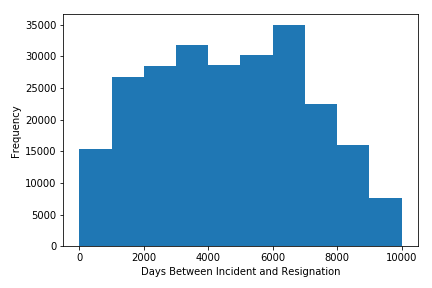
\includegraphics[width=0.5\textwidth]{complaint1.png}
\end{figure}

\begin{figure}[h!]
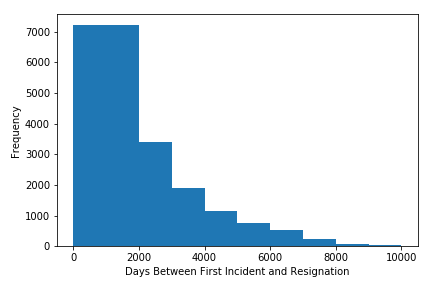
\includegraphics[width=0.5\textwidth]{complaint2.png}
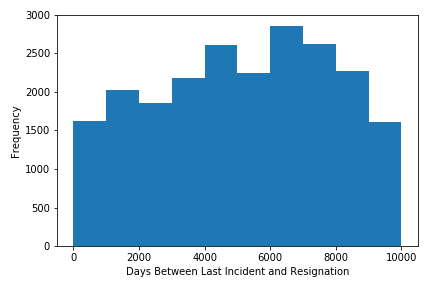
\includegraphics[width=0.5\textwidth]{complaint3.png}
\end{figure}

\FloatBarrier
\section{Data Integration}

In this section we used Trifacta to join the complaint and settlement databases. The first topic we looked into was the relationship between neighborhood income and settlements. For this first query however, we needed to use the postgis geographic objects and so did not use Trifacta. We joined the data area table to the settlement table based on whether the settlement lat/long falls within a community, then grouped by the community and summed the settlements. In order to add them however, we would need to go through each individual claim and see if we can determine a location based on the description, or go through the officers, which may not be accurate. It is a bit easier to see this data in plot form, so below are two plots. There isn't a clear distribution here. It looks like higher income neighborhoods have less settlements, which would make sense, as nicer neighborhoods generally have less crime. However it also appears some of the lowest income neighborhoods
also have less settlements. It's possible that citizens in these neighborhoods are unable to afford a lawyer and as such do not go through with the process, but I'm not sure that that cost falls on them to begin with.

\begin{figure}[h!]
\centering
\caption{Settlements per Neighborhood}
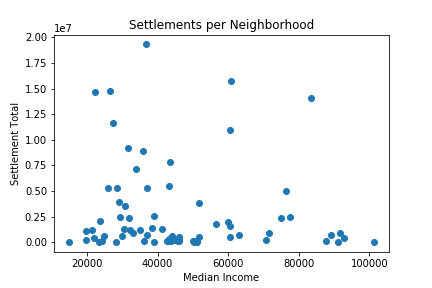
\includegraphics[width=0.45\textwidth]{settle1.png}
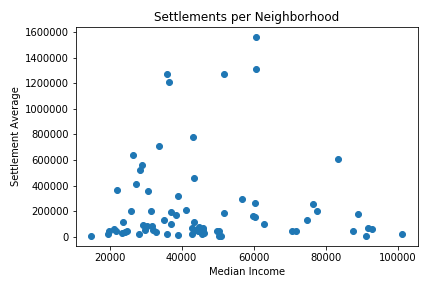
\includegraphics[width=0.45\textwidth]{settle2.png}
\end{figure}

The second question we explored was the settlement cost by officer race. To start, we looked at the races of the officers and got some statistics for the settlement cost for each officer by joining the settlement information with a table with the settlement id. Using Trifacta we grouped the information by race of the officer. We could then create columns for each of the races. The averages listed are only for settlements less than a million. This was to get a better understanding of what occurs in the typical case of a settlement without any large outliers. The table of average settlement values is below (figure 3). The average white officer settlement costs the department around 81k which is 10k more than any other race. I would guess that when a white officer is involved, the police might pay out slightly larger settlements to somewhat avoid the bad press behind any
race-related issues. 

\begin{figure}[h!]
\centering
\caption{Table of Settlement Costs}
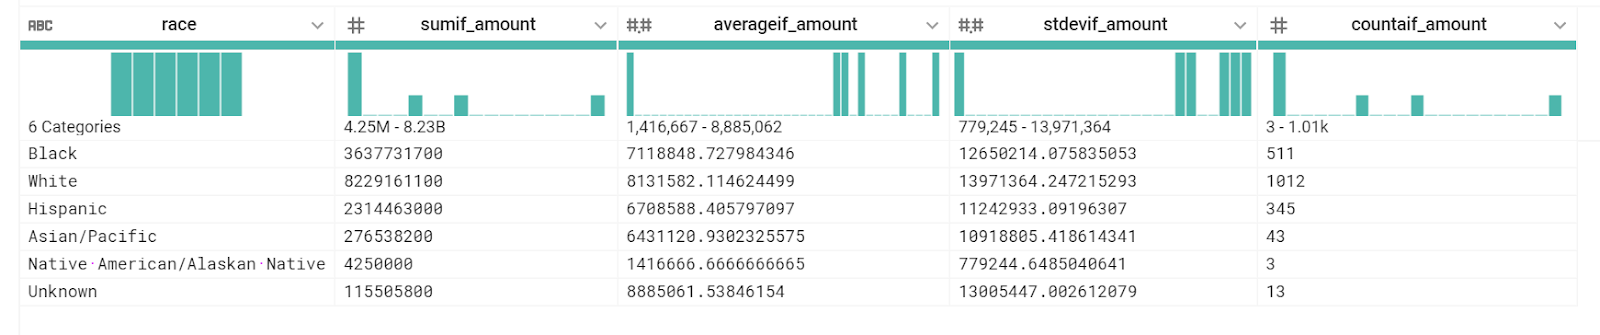
\includegraphics[width=0.85\textwidth]{RaceTable.PNG}
\end{figure}

The third question was to analyze officer age during the time of a settlement. Using Trifacta we were able to find out that this value was around 39.56 years old. For comparison, the average age of current officers in CPD is 44.5 years old, although we do expect younger officers are more likely to be in the field and thus be involved in complaints/settlements. Below is the average age by rank for current officers, showing that lower ranks tend to be younger. in settlements, so it does seem that younger officers in general are more likely to be involved in an incident.

\begin{figure}[h!]
\centering
\caption{Officer Ages}
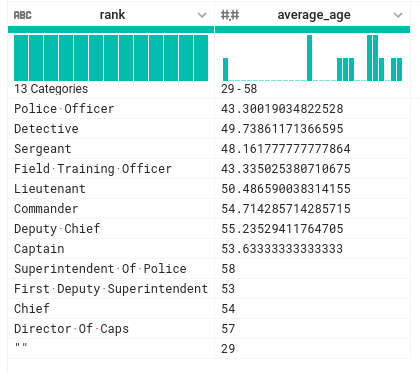
\includegraphics[width=0.85\textwidth]{ages.png}
\end{figure}

The last point we looked into was the correlation between complaints and settlements. Similar to the first question we used postgis to put the allegations and settlements into each neighborhood and counted them. For the most part, there seems to be a strong correlation between the two---as the number of allegations decreases, so does the number of settlements. There are quite a few inconsistencies however. Looking at the first few, the Loop stands out as having a lot of allegations and few settlements, while North Lawndale shows the opposite. The Loop is an interesting neighborhood in that it is extremely populated during the day with tourists and people going to work, but most do not actually live in the Loop. It might make sense that a person in the Loop would submit a complaint, but then maybe not stick around to follow through with court procedures. From the plot below, the Loop (bottom right) looks like it might be an outlier, but the rest of the neighborhoods do follow a roughly linear distribution.

\begin{figure}[h!]
\centering
\caption{Allegations vs Settlements}
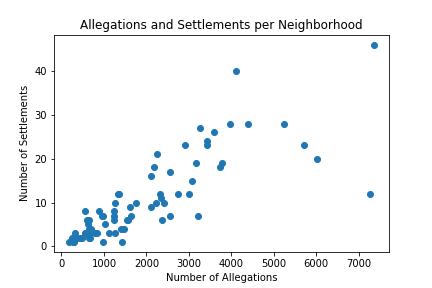
\includegraphics[width=0.45\textwidth]{alleg_scatter.png}
\end{figure}

\FloatBarrier
\section{Workflow Analytics}

In this section we used Spark to work with the database and create visualizations. The first task we tackled was to cluster officers before and after being involved in a settlement. We used features of rank, race, gender, age, number of complaints, and number of awards. The after clustering also used the number of settlements. The main takeaways here were that the most important features for clustering were age, number of complaints, and number of awards. Rank was also somewhat important, but it also is highly correlated with age and so somewhat redundant. Gender and race had little impact on the clusters. In the future it would be nice to have some way to map officers from before to after and so identify segments of the officer population that are more at risk of repeat offending versus those that behave well after a settlement.

\begin{figure}[h!]
\centering
\caption{Clustering careers before and after settlement}
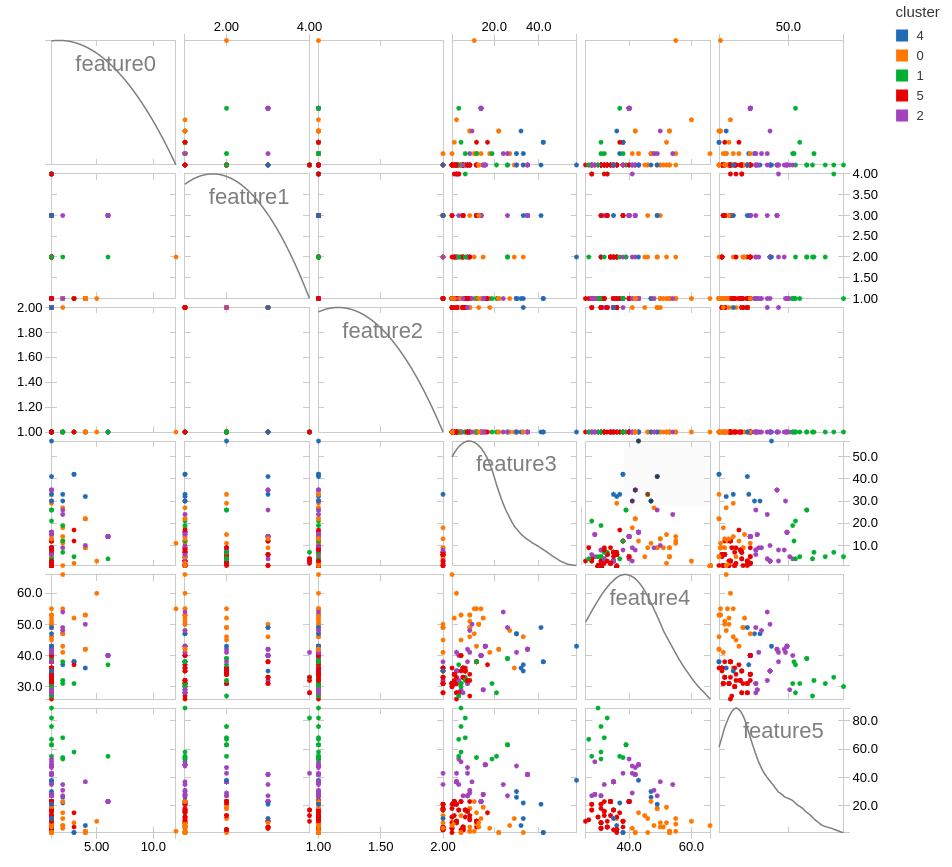
\includegraphics[width=0.45\textwidth]{cluster.png}
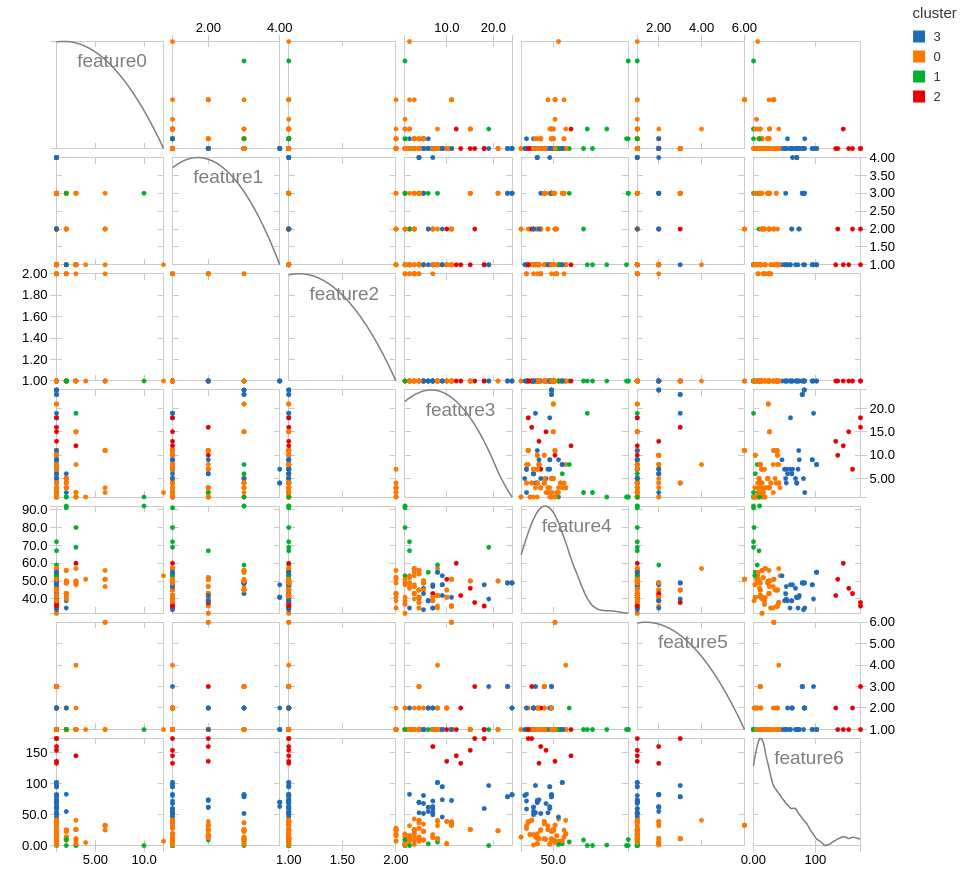
\includegraphics[width=0.45\textwidth]{cluster2.png}
\end{figure}

The second question that we looked into here was to quantify whether officers got fewer or more complaints after being involved in a settlement. The first plot on the left shows that officers involved in settlements do in fact get fewer complaints afterwards, averaging 10 before and 4 after. Conversely, these officers get more awards after the settlement, increasing from 19 before to 24 afterwards. If officers were being fired or assigned to desk duty after a settlement we expect they would most likely get fewer awards, so the combination of fewer complaints and more awards seems to imply that the officers affected are in fact changing their behavior for the better.

\begin{figure}[h!]
\caption{Number of Complaints and Awards After Settlement}
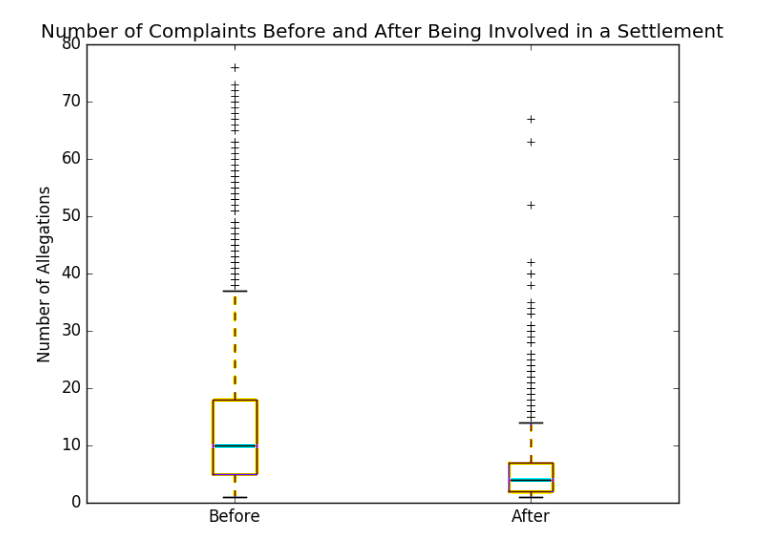
\includegraphics[width=0.5\textwidth]{settb.png}
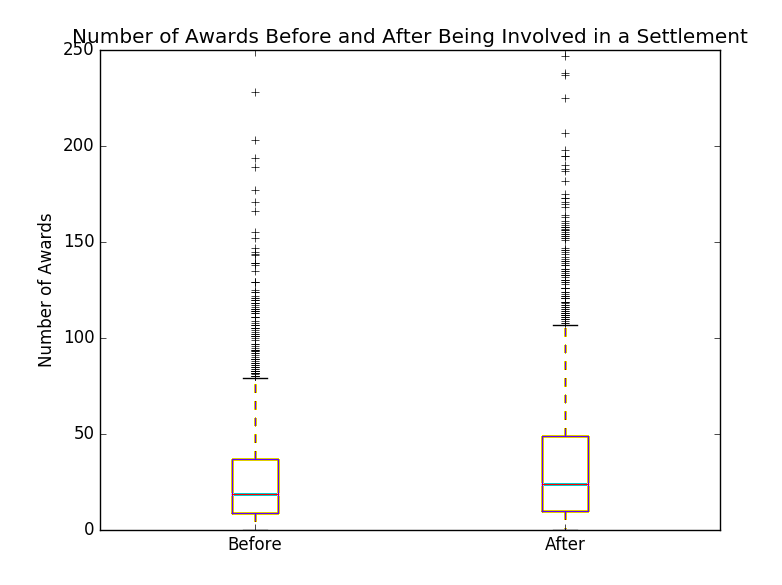
\includegraphics[width=0.5\textwidth]{awards.png}
\end{figure}

The final topic we looked at was whether neighborhoods see fewer complaints after a settlement occurs. The data however, was a bit sparse here, and so we could not draw any definitive conclusions. We did see an overall 49\% decrease in complaints in the neighborhood that a settlement took place, perhaps indicating that overall happiness with the police increases or overall crime decreases.

\FloatBarrier
\section{Machine Learning}

We continued to use Spark for this checkpoint, using its machine learning library to make predictions. The first prediction we attempted to make was to predict which officers would receive a complaint in a given year. We created a decision tree classifier with features of age, rank, race, and number of complaints prior to 2017. From there we attempted to predict who would receive a complaint in 2017. We got an accuracy of 97\% which sounds good, but digging into the data revealed some problems. In 2017 there are approximately 11,000 active officers, of which only about 300 received a complaint. So the model mostly predicts 0 complaints, and only correctly predicts a few officers. It does however output some interesting probabilities, showing that the average officers has a 4\% chance of getting a complaint in a given year. This rate jumps to 20\% though for officers with 12 complaints. In the future it might work better to predict over an entire career instead of just a year.


The second prediction we worked on was predicting settlement values. We used features of officer age, race, gender, number of complaints, number of settlements, and value of those settlements. We used a generalized linear model with a log-gaussian fit. The results are similar in distribution to the actual values, so the model preforms well. It does work much better with the smaller settlement values that the large ones, which is to be expected given that there aren't many large values in the data and so the model doesn't have much to work with.

\begin{figure}[h]
\caption{Predicted and Actual Settlement Values}
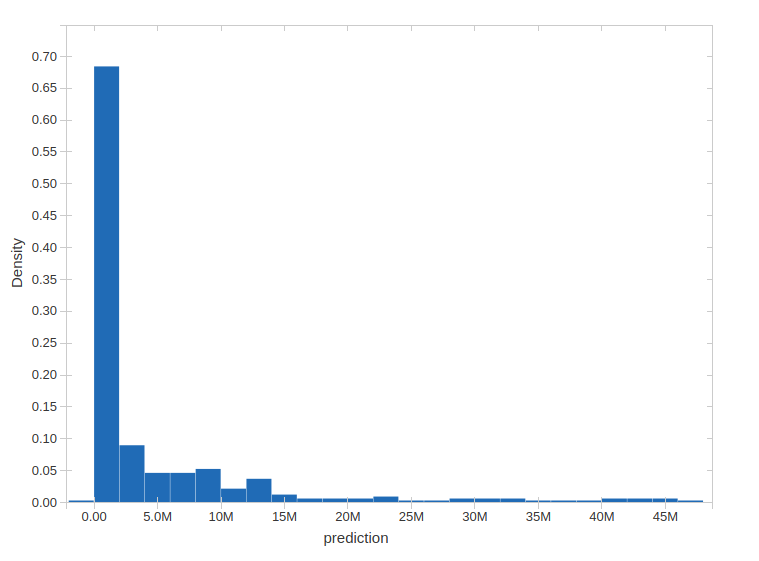
\includegraphics[width=0.5\textwidth]{predicted.png}
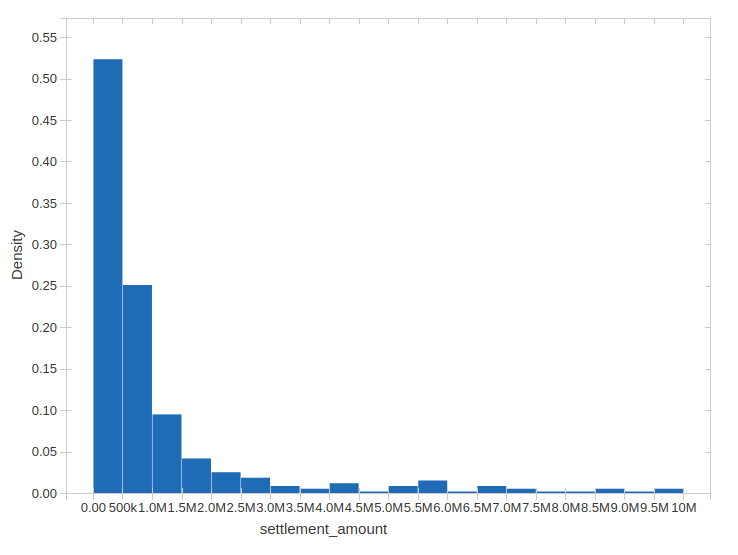
\includegraphics[width=0.5\textwidth]{actual2.png}
\end{figure}

\FloatBarrier
\section{Neural Nets}

We started by creating a table of officer data and salaries from 2017. We specifically only take one year, as including an officers previous years salary probably gives away the current salary, which would make the neural net mostly useless. One hot encoding is used for the categorical variables which worked better than simply inputing category codes. The neural net uses 3 hidden layers with ReLu activation. The test data has a mean absolute error of \$3350, which, for salaries roughly \$50k-180k, isn't bad. We tested a few different configurations but consistently got the best results with the above setup. Looking at the plot of actual vs predicted salaries, it seems to do pretty well with most sections of the spectrum of salaries and there are no clear mismatched areas.
Certain features such as rank tend to be better predictors of salary
When removing the rank of officers in predictor, mean squared error increase to \$5500. Other features alone do not significantly affect the performance. In the future, more tests can be done to help determine the optimal combination of features.

\begin{figure}[h]
\caption{Predicted and Actual Settlement Values}
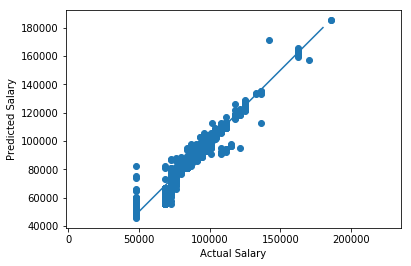
\includegraphics[width=0.5\textwidth]{pred.png}
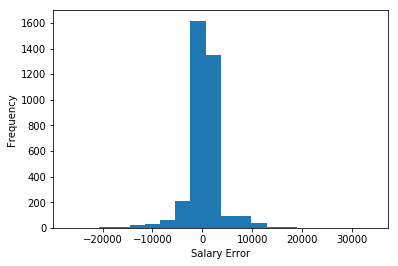
\includegraphics[width=0.5\textwidth]{error.png}
\end{figure}

\FloatBarrier
\section{Visualization}

Lastly, we visualized a couple of our hypotheses in Tableau and D3 to get a better understanding of our findings. The first thing that we looked into was the number of allegations per capita in the neighbourhoods of Chicago. The allegations per capita is similar across the board, with a few neighborhoods standing out. First and foremost is Fuller Park, the only neighborhood in red in the first map, as it has almost as many complaints as residents (around 2,000). Excluding Fuller Park we can see that a few other neighborhoods have elevated complaint levels, namely the Loop and a few west and south side areas. The Loop has lots of traffic, and the other neighborhood are rougher areas, so it makes sense that they have more complaints per capita.

\begin{figure}[h]
\caption{Allegations per Capita (with and without Fuller Park)}
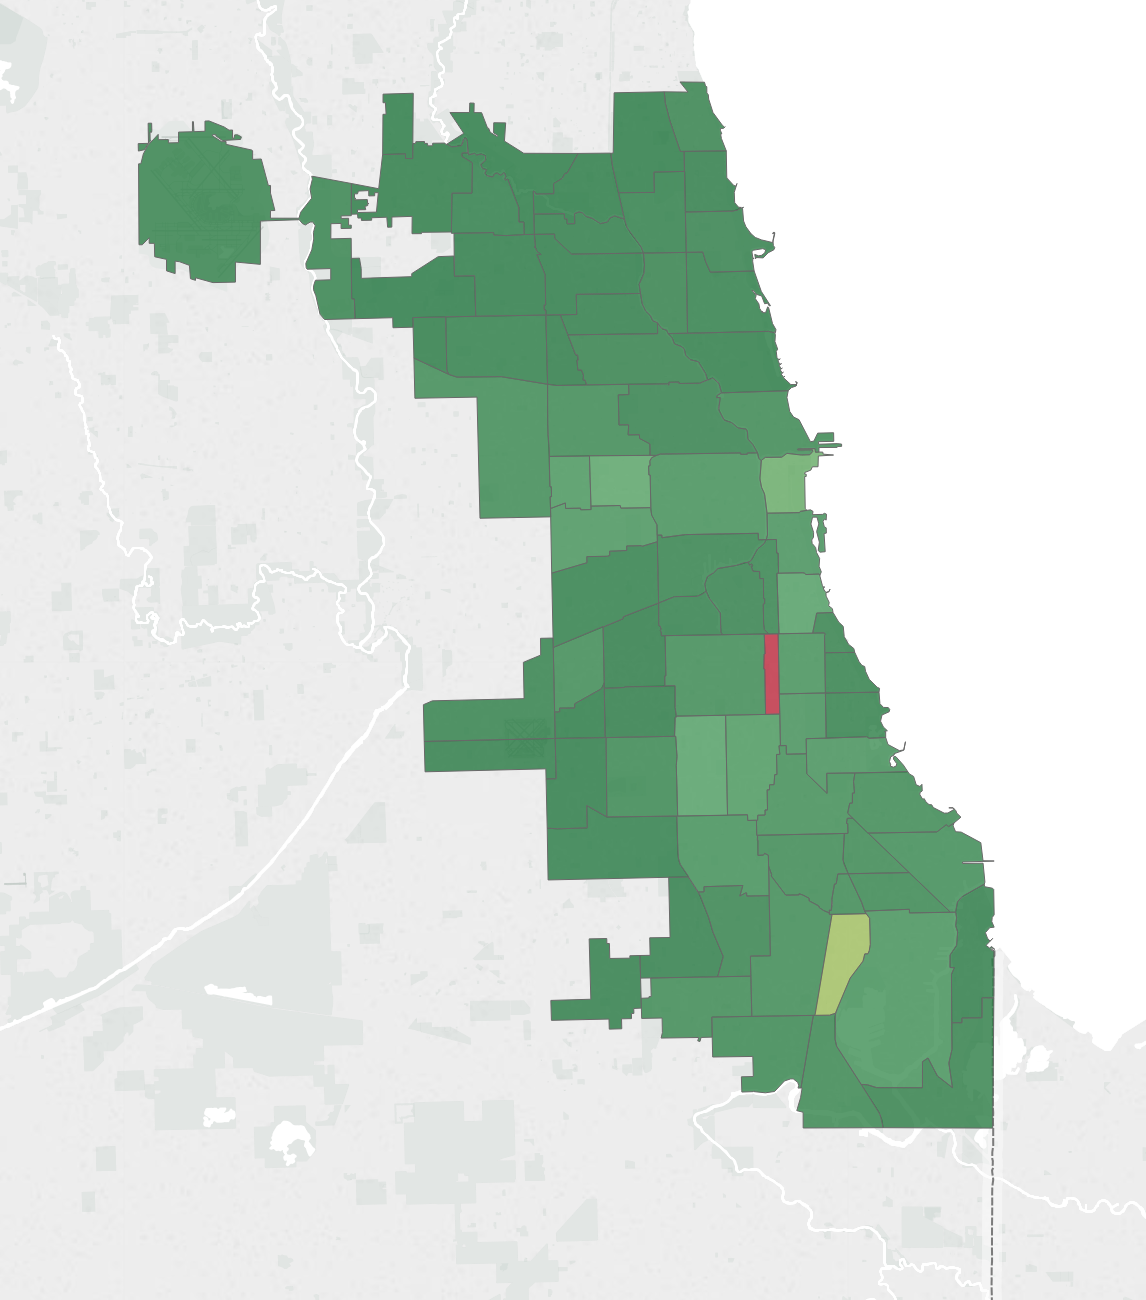
\includegraphics[width=0.5\textwidth]{plot1.png}
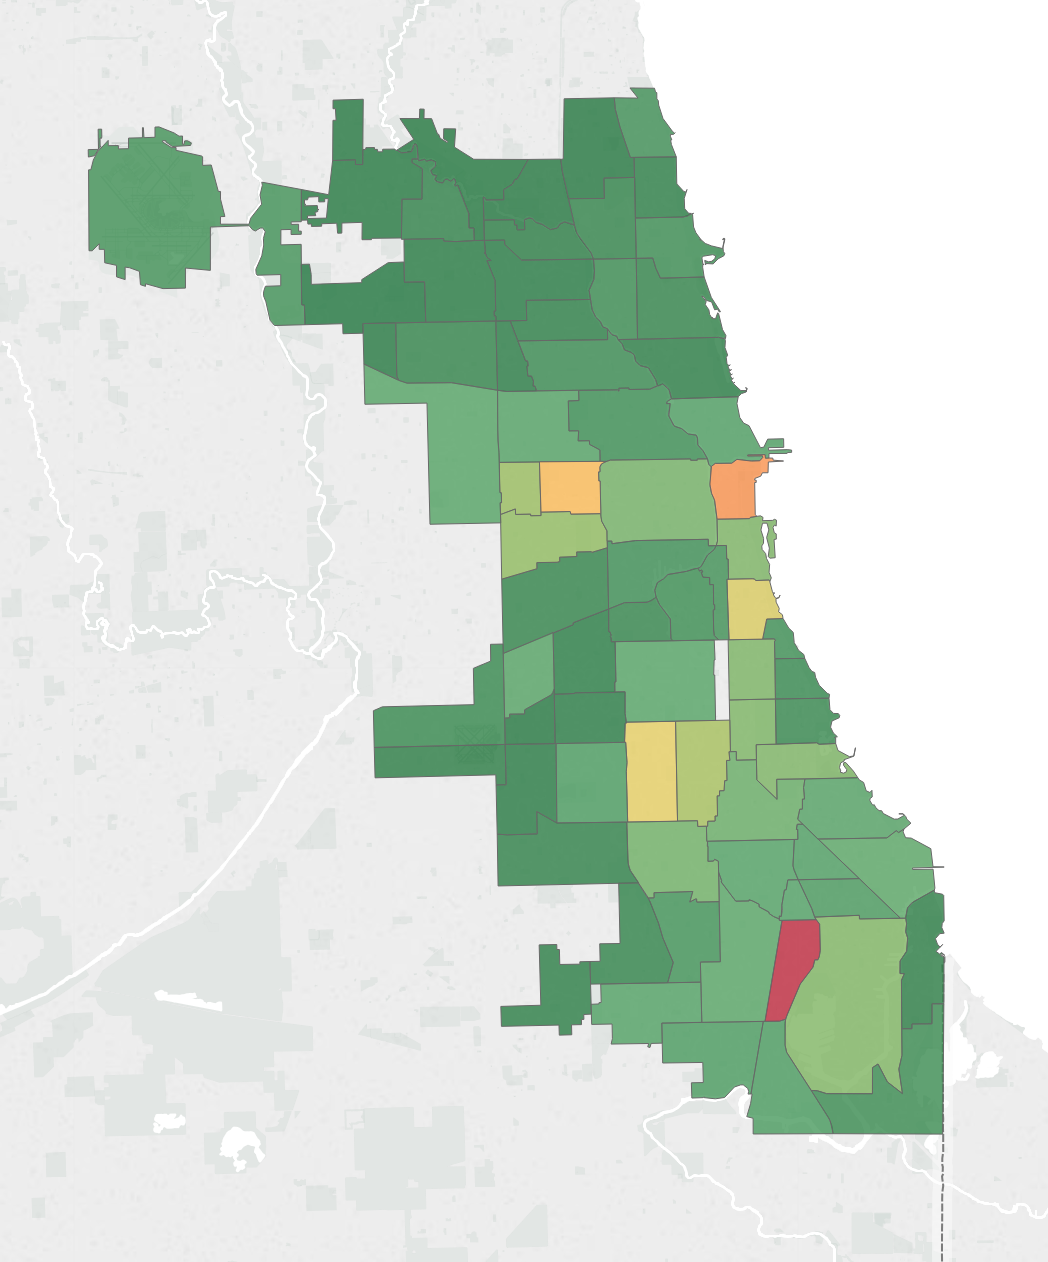
\includegraphics[width=0.5\textwidth]{plot2.png}
\end{figure}

Next, we plotted a relation between the median income in the neighbourhoods to the number of allegations in each of them. This plot is pretty similar to the number of settlements per neighborhood plot we made in an earlier checkpoint. There are a few outliers, the Loop and Austin, and presumably some spillover from the Loop in the Near West and Near North Side. Excluding those, it looks like generally, the number of complaints is inversely correlated with median income. There are some neighborhood with low incomes that also don’t report many complaints. It’s possible these neighborhoods don’t believe the police will help and are thus under reported, but it would be hard to prove this without further analysis. In addition, neighborhoods such as the Loop and Near West Side may over report for allegations for many things that may not really classify as allegation due to the nature of these wealthier areas. However more analysis on the types of analysis done would be required.


\begin{figure}[h]
\centering
\caption{Neighborhood median income vs number of allegations}
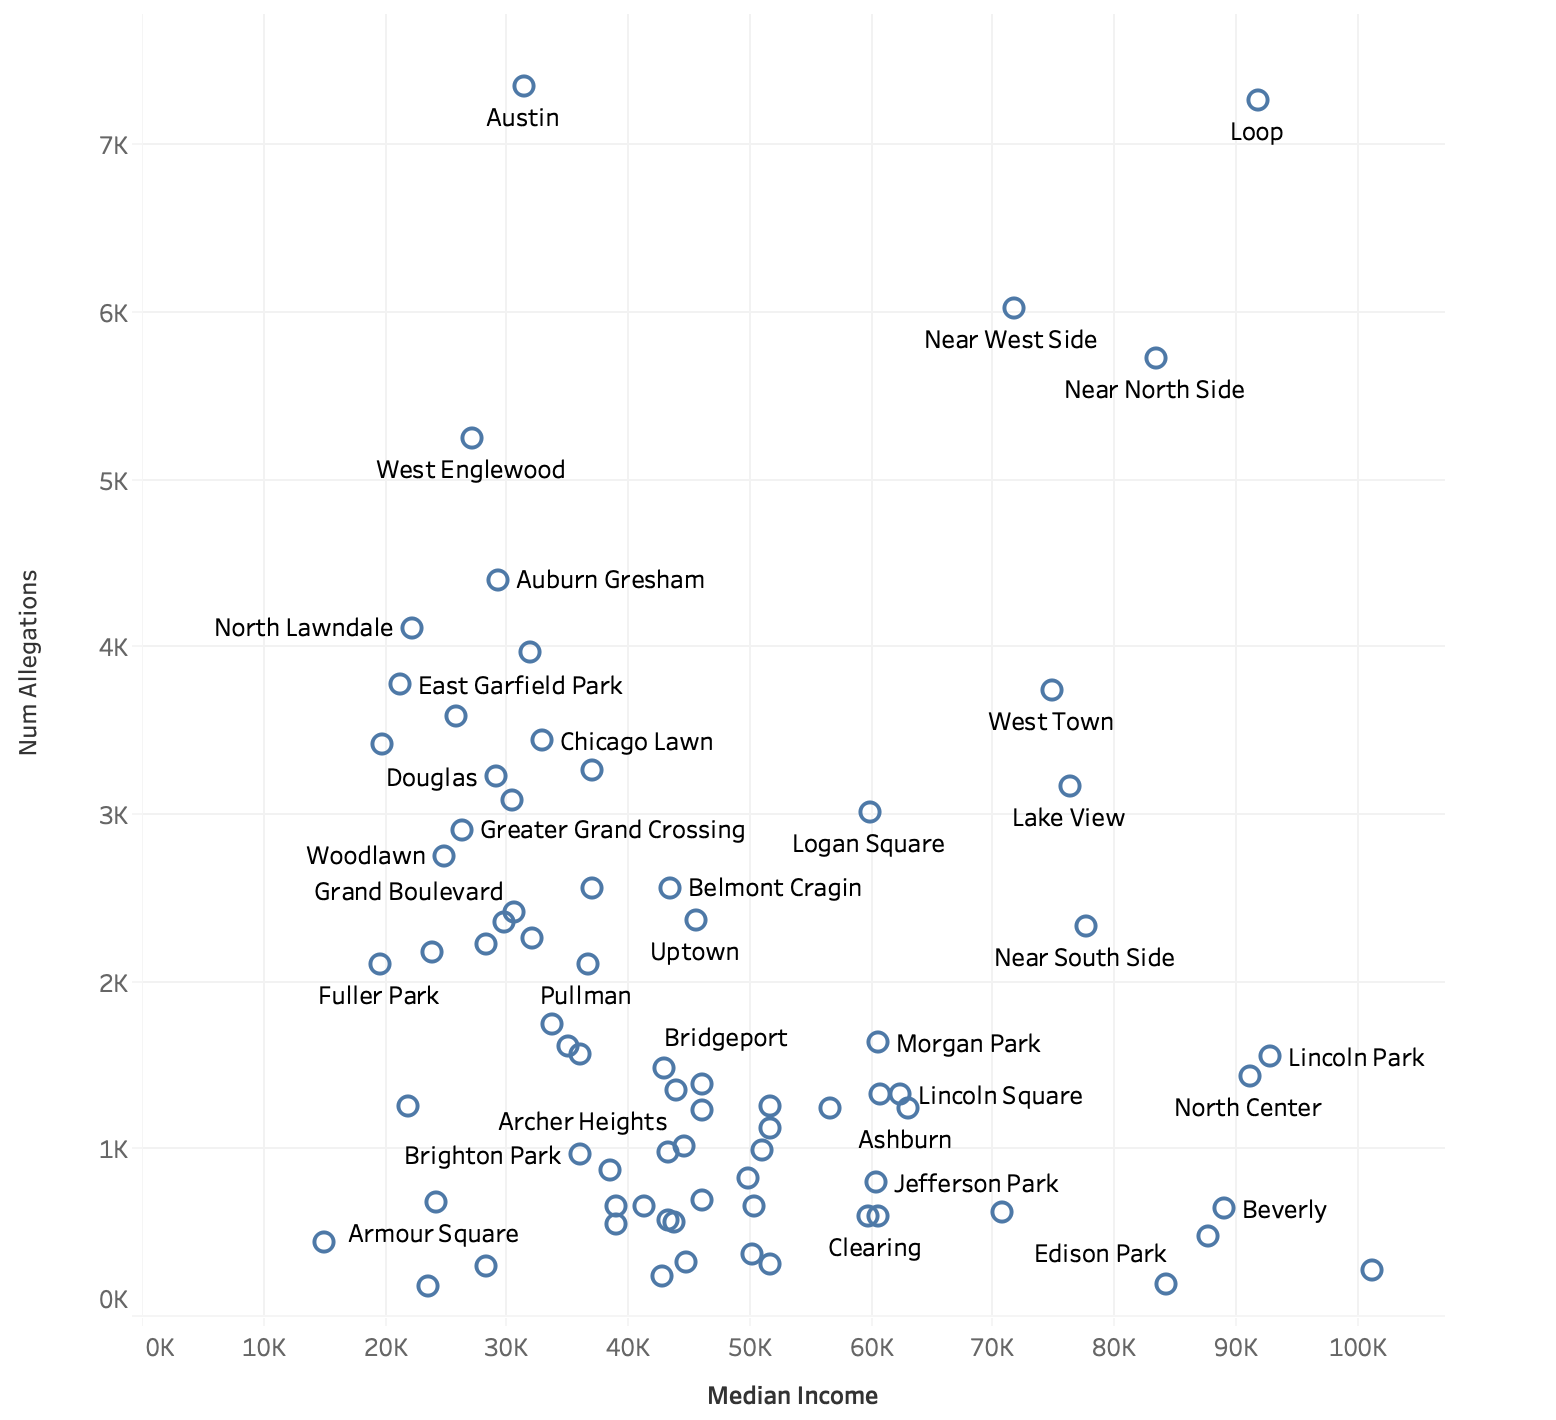
\includegraphics[width=0.75\textwidth]{scatter.png}
\end{figure}

The last visualization we created looks at the average cost of officers separated by their complaint quartiles. The cost is defined as each officer's salary plus any portion of a settlement they were involved in for that year. The first quartile consists of officer who have 2 complaints or less, with an average of 0.64 complaints. The second quartile is officer with 2 to 7 complaints, with an average of 4.94 complaints. The third quartile is officers with 7 to 15 complaints, with an average of 11, and the last quartile has up to 175 complaints, with 27.9 complaints per officer on average. Overall we can see that officers with more complaints generally cost the department more. The noticeable dip in the first quartile is most likely due to the hiring of a many new officers.

\begin{figure}[h]
\caption{Cost of Officers from 2002-2017}
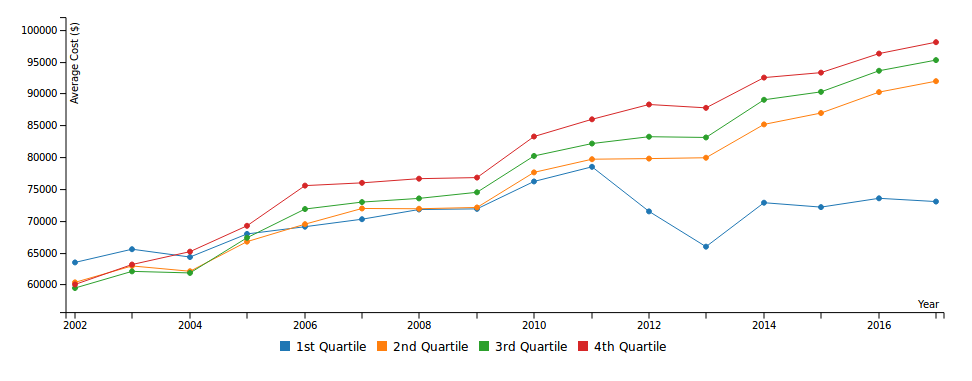
\includegraphics[width=\textwidth]{costline.png}
\end{figure}

\FloatBarrier
\section{Conclusion}

For our project, we were ultimately able to make a few conclusions. Our first conclusion is that officer salary is independent of neighborhood, as it varies mostly by rank as opposed to where they work. This presumably encourages officers to behave similarly in every district across the city. We also found that officer race is not a very strong predictor of the officers salary. In terms of officer behavior, officers that remain on the force after a settlement tend to have more awards and few allegations against them, hopefully meaning they are generally behaving better. We also saw that officers with more complaints cost the force more per year on average than officers with fewer complaints. Finally, after removing outliers, the number of allegations is loosely inversely correlated with the median income of the neighborhood. To strengthen this study in the future, analysis on the firings and suspensions should be looked into. Suspensions and firings potentially cost individual officers their salary, and cost the unit manpower, so looking into these results would help to bolster our analysis. 

\end{document}